%!TEX root = report.tex
\exercise{2D wavelet transforms}
As \cite[p. 501]{gonzalez2002digital} suggests, it seems easy to extend the one-dimensional transforms to two-dimensional transforms.
However, really understanding what happens in 2D proved to be quite laboursome, and in the process we took multiple detours.\footnote{It also retroactively helped understanding the one-dimensional transform quite a lot better.}

In this section, the two-dimensional discrete Haar wavelet transform, and its inverse, are implemented and explained.
The transforms will also be applied to an image of a vase.

\subsection{\texorpdfstring{2D \(J\)-scale DWT}{2D J-scale DWT}}
Much as the one-dimensional transform depended on \texttt{decompose}, the two-dimensional transform depends on the \texttt{decompose\_2d} function.
This function receives as input variables an \texttt{image}, and a string, \texttt{along}, which indicates in which direction the decomposition should take place.
\matlabexternal{../decompose_2d.m}
This is very similar to the one-dimensional case.
The only difference is that the operation is performed for all rows or columns in the image.

The two-dimensional scaling function and wavelets are listed \cite[Eq 7.5-1 through 7.5-4]{gonzalez2002digital}.
The tricky part\footnote{For us, that is.} was not \emph{understanding} those functions, but understanding what these functions mean for the \emph{implementation}.
The scaling functions are built by combining the four one-dimensional functions:
\begin{itemize}
	\item \(\varphi(x)\): Scaling along the \(x\)-axis. Corresponds to taking the approximation part along the \(x\)-axis.
	\item \(\psi(x)\): Wavelet along the \(x\)-axis. Corresponds to taking the detailed part of the decomposition along the \(x\)-axis.
	\item Equivalent functions for \(y\).
\end{itemize}
E.g., \cite[Eq. 7.5-2]{gonzalez2002digital}, for the horizontal detail component, reads:
\[\psi^H(x, y) = \psi(x)\varphi(y)\]
For the implementation, this roughly means that the image first has to be decomposed along the \(y\)-axis, and the approximation\footnote{Because it says \(\varphi(y)\), which is the scaling function.} part of that decomposition must be further decomposed along the \(x\)-axis, and the resulting detailed\footnote{Because it says \(\psi(x)\), which is the wavelet function.} part will be \(\psi^H(x, y)\), the horizontal details.

A comprehensive overview of the full transformation is depicted in \cite[Figure 7.24(a)]{gonzalez2002digital}.

Using this method for the two-dimensional scaling and wavelet functions, the following function has been implemented:
\matlabexternal{../IPdwt2.m}
As in the one-dimensional case, the function is recursive, to reflect the recursive nature of the representation.
In the process of going deeper in the recursion, more and more parts of the DWT representation are set in \texttt{finalImage}, starting with the finest details in the top-right, bottom-right and bottom-left parts, and proceeding with the top-left part in the recursion.

\subsection{Contrast-stretching of wavelet coefficients}
To enhance the visibility of the detail parts, the contrast of these parts can be stretched to the same range as the original image.
This will greatly improve the visibility, since the detail parts have much smaller values, since they are just the small differences between the approximations of different levels. In addition to that they are \emph{small}, the differences can also be \emph{negative}.

To realise the contrast stretching, the function \texttt{IPdwt2scale} has been implemented and listed below. This function is once again recursive, since each detail part (there are \(3\cdot2^J\)) generally has a different maximum value. Especially the diagonal detail parts have much lower values than the horizontal and vertical detail parts.
\matlabexternal{../IPdwt2scale.m}
The function stretches the contrast of each of the currently finest detail level individually, and then proceeds to the coarser detail levels, if any. \texttt{IPdwt2scale} needs the input variable \texttt{approxSize} to detect when it has reached the base case of the recursion, since it shouldn't stretch the contrast of the approximation part of the DWT representation.

\subsection{Transforming a vase}
The transformation has been applied to \texttt{vase.tif}, using \(J=3\).
After applying \texttt{IPdwt2scale} to the result, the image in Figure~\ref{fig:vase_dwt} was obtained:
\begin{figure}[htb]
 \centering
 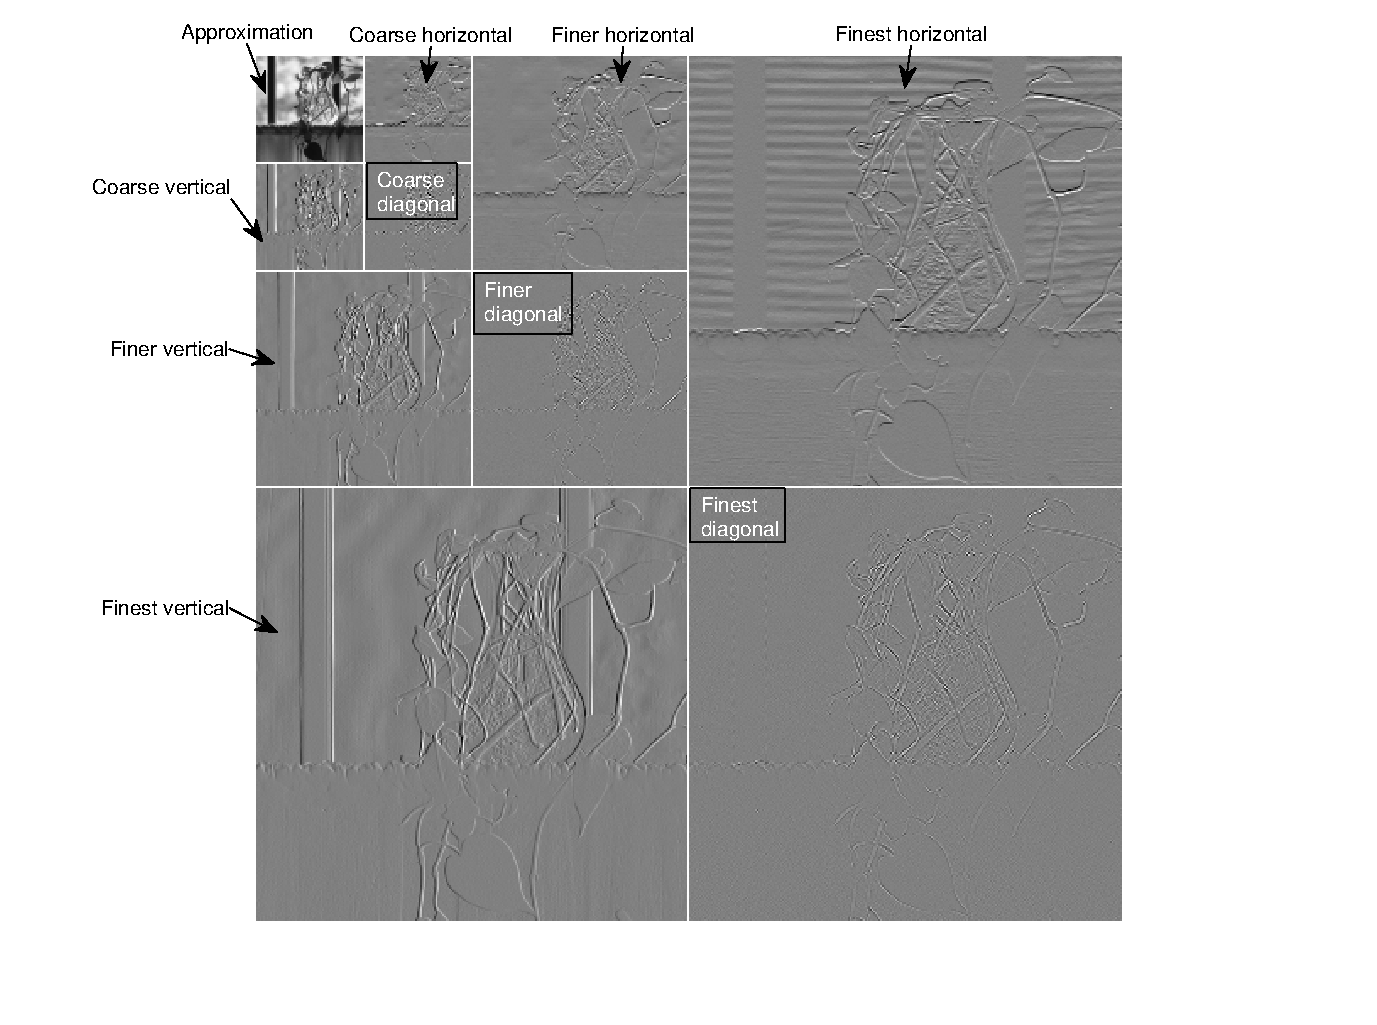
\includegraphics[width=\linewidth]{labeled_vase_dwt.eps}
 \caption{The DWT representation of \texttt{vase.tif}.}
 \label{fig:vase_dwt}
\end{figure}

\clearpage

\subsection{\texorpdfstring{2D inverse \(J\)-scale DWT}{2D inverse J-scale DWT}}
Just like the one-dimensional transformation, the two-dimensional transformation is also invertible.
Mirroring the implementation in \texttt{IPidwt}, \texttt{IPidwt2} depends on the function \texttt{compose\_2d}:
\matlabexternal{../compose_2d.m}
What this function does should be clear by now: Along the specified axis, it assigns to the even elements the approximation \emph{plus} the details, and to the odd elements the approximation \emph{minus} the details.

\texttt{compose\_2d} has been utilized by \texttt{IPidwt2}, to implement the two-dimensional inverse DWT:
\matlabexternal{../IPidwt2.m}
This recursive function combines the current approximation with the currently coarsest details to compose the finer approximation.
The result is passed along to a deeper recursion with a smaller \texttt{J}.
This process stops once texttt{J} has reached 0.

Applying this \texttt{IPidwt2} to the result of \texttt{IPdwt2}\footnote{So not the contrast stretched image!} with the same \texttt{J = 3} (or any other \(1 \leq \texttt{J} \leq 9\)), yields the image in Figure~\ref{fig:vase_restored}. This image should be familiar, since it is exactly equal to the input image, \texttt{vase.tif}.

\begin{figure}[htb]
 \centering
 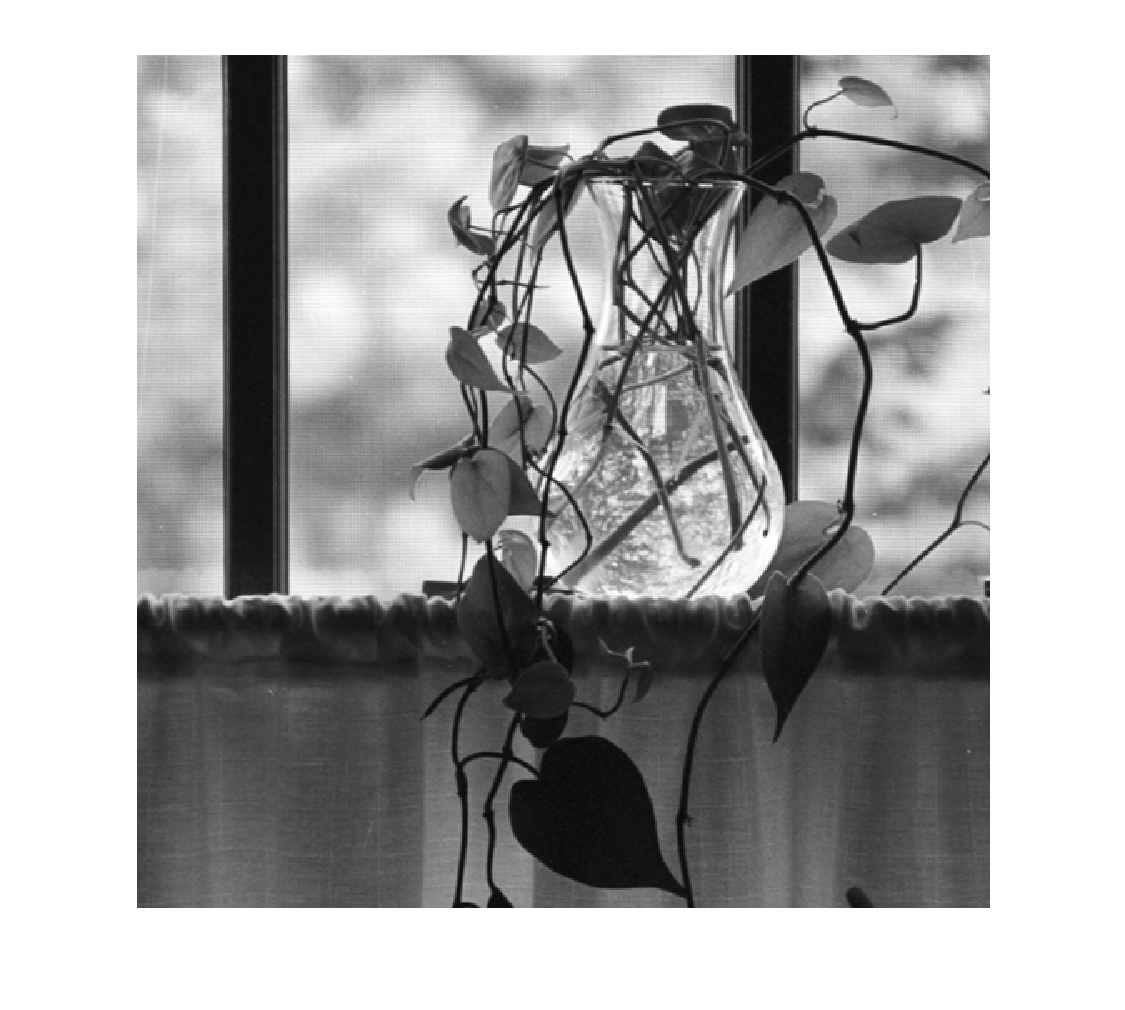
\includegraphics[width=\linewidth]{vase_restored.eps}
 \caption{This image shows that the decomposed vase has been carefully restored to a proper vase, without losing any pieces. (Even the water is still in there!)}
 \label{fig:vase_restored}
\end{figure}

\clearpage